\documentclass[a4paper]{article}
\usepackage[margin=1in]{geometry} % 设置边距,符合Word设定
\usepackage{ctex}
\usepackage{graphicx} %插入图片的宏包
\usepackage{float} %设置图片浮动位置的宏包
\usepackage{subfigure} %插入多图时用子图显示的宏包
\usepackage{lipsum}
\usepackage{minted}% 语法高亮和代码样式设置方面更加强大和灵活
\usepackage{listings}% 引入listings包,用于在文档中插入代码,并可自定义代码样式
\usepackage{caption}
\usepackage{subfigure}% 并排插入图片
% 表格宏包:
\usepackage{booktabs}  %% 三线表
\usepackage{diagbox}   %% 斜线表头
\usepackage{multirow}  %% 合并单元格


\title{奥运会项目评估模型:随机森林回归在体育决策中的应用}
\author{ Guo Runheng,\ Yang Zicheng,\ Qiu Xinyang}
\date{\today}

\begin{document}
    \maketitle


\begin{abstract}
    % 奥运会项目调整是奥运会持续发展的重要方式,对奥运会项目的调整有利于提升奥运会的社会与时代价值。本文主要采用随机森林回归模型,对未来奥运会项目的增减进行了评估与预测。
    % \par 针对任务1,我们根据IOC标准,通过在网上查找多方面的资料并参考权威数据,对这些运动的受欢迎度和可达性、性别平等性、可持续性、包容性、相关性与创新性、安全与公平竞争性、新建更多项目的可能性共七个维度因素,在0-1之间进行了评分。
	% \par 针对任务2,我们对1948-2020年项目数量的变化表格进行分析,利用Python语言进行了数据的可视化操作。然后,我们使用一次线性拟合,分析从1948到2020年的项目数变化的规律性特征。然后,我们以七个维度因素作为自变量,线性拟合的斜率作为因变量,训练了一个随机森林回归模型。
    % \par 针对任务4,我们利用训练好的随机森林回归模型,识别了三个可能在2032年布里斯班奥运会上新增或重新引入的 SDEs ,并确定其优先推荐的顺序。
    The adjustment of Olympic SDEs is an important way for the continuous development of the Olympic Games. Adjusting the Olympic SDEs is conducive to enhancing the social and contemporary value of the Olympics. This paper mainly uses the random forest regression model to evaluate and predict the increase or decrease of future Olympic SDEs.
    \par For Task 1, based on the IOC standards, we searched for a variety of information online and referred to authoritative data to score these sports on seven dimensions: popularity and accessibility, gender equality, sustainability, inclusivity, relevance and innovation, safety and fair competition, and the possibility of creating more events.
    \par For Task 2, we analyzed the table of event numbers from 1948 to 2020 and used the Python language for data visualization. Then, we performed a linear fit to analyze the regularity of the changes in the number of events from 1948 to 2020. Subsequently, we trained a random forest regression model using the seven dimensions as independent variables and the slope of the linear fit as the dependent variable.
    \par For Task 3, we utilized the well-trained random forest regression model to identify three SDEs that may be added or reintroduced at the 2032 Brisbane Olympic Games and determined their priority recommendation order.
\end{abstract}
\tableofcontents
\section{Introduction}

\subsection{Background}  
The adjustment of Olympic SDEs plays a vital role in the development of the Olympic Games, allowing the Olympics to keep pace with the social and contemporary needs. Data shows trend of SDEs' changes, while IOC also gives its criteria for sports inclution. To better evaluate SDE's addition and reduction, we need to figure out inner relationship between IOC criteria and SDE's changes.

(来两张图吧,别人这段都有图表的,参照《2021年美赛特等奖原版论文集》)
\subsection{Restatement of the Problems}
\begin{itemize}
\item[$\bullet$]List and describe the various factors your team identifies that need to be
considered when addressing the IOC criteria. Note that factors may be quantitative or qualitative,
constant or variable, and deterministic or probabilistic. Be sure to justify your choices.
\item[$\bullet$]Use your factors to build a model (or set of models) to help the IOC evaluate
which SDEs align best with Olympic criteria. Test your model on at least three SDEs that have been added or removed from recent
Olympics, namely Olympic years 2020, 2024, and 2028 and at least three SDEs that have
continuously been in the Olympic programme since the 1988 games or earlier. The
supplied data provides information about which sports and
disciplines, and number of events, have appeared in each Olympics since their modern
formation. Be sure to highlight the general applicability of your model by choosing a
diverse collection of SDEs to evaluate. Discuss how your model affirms these SDEs’
current Olympic status.
\item[$\bullet$]Identify three SDEs that could be new additions or reintroductions for the 2032 Olympics
in Brisbane. Make sure to identify which SDE should be considered first, second and
third for inclusion in the Brisbane games. Are there any SDEs that you believe have
potential for inclusion in an Olympic games in 2036 or beyond?
\end{itemize}
\subsection{Data Pre-processing}
We first excluded some items with poor data, such as polo, rackets and karate, choosing data from 33 items to train our model (20\% of them are randomly decided as test dataset for model, and two of them are for manually test).
We then used linear fit to the number of projects from 1948 to 2020 for each project. Figure 1 shows the result of linear fit. 
Discovering that the intercept of figure 1 is suitable for evaluating new or old SDEs, we generated figure 2, whose y axis shows the intercept of figure 1,
and x axis represents the increasing rate of each SDE.
\captionsetup[listing]{labelformat=empty}
\begin{figure}[h] %H为当前位置,!htb为忽略美学标准,htbp为浮动图形
    \centering %图片居中
    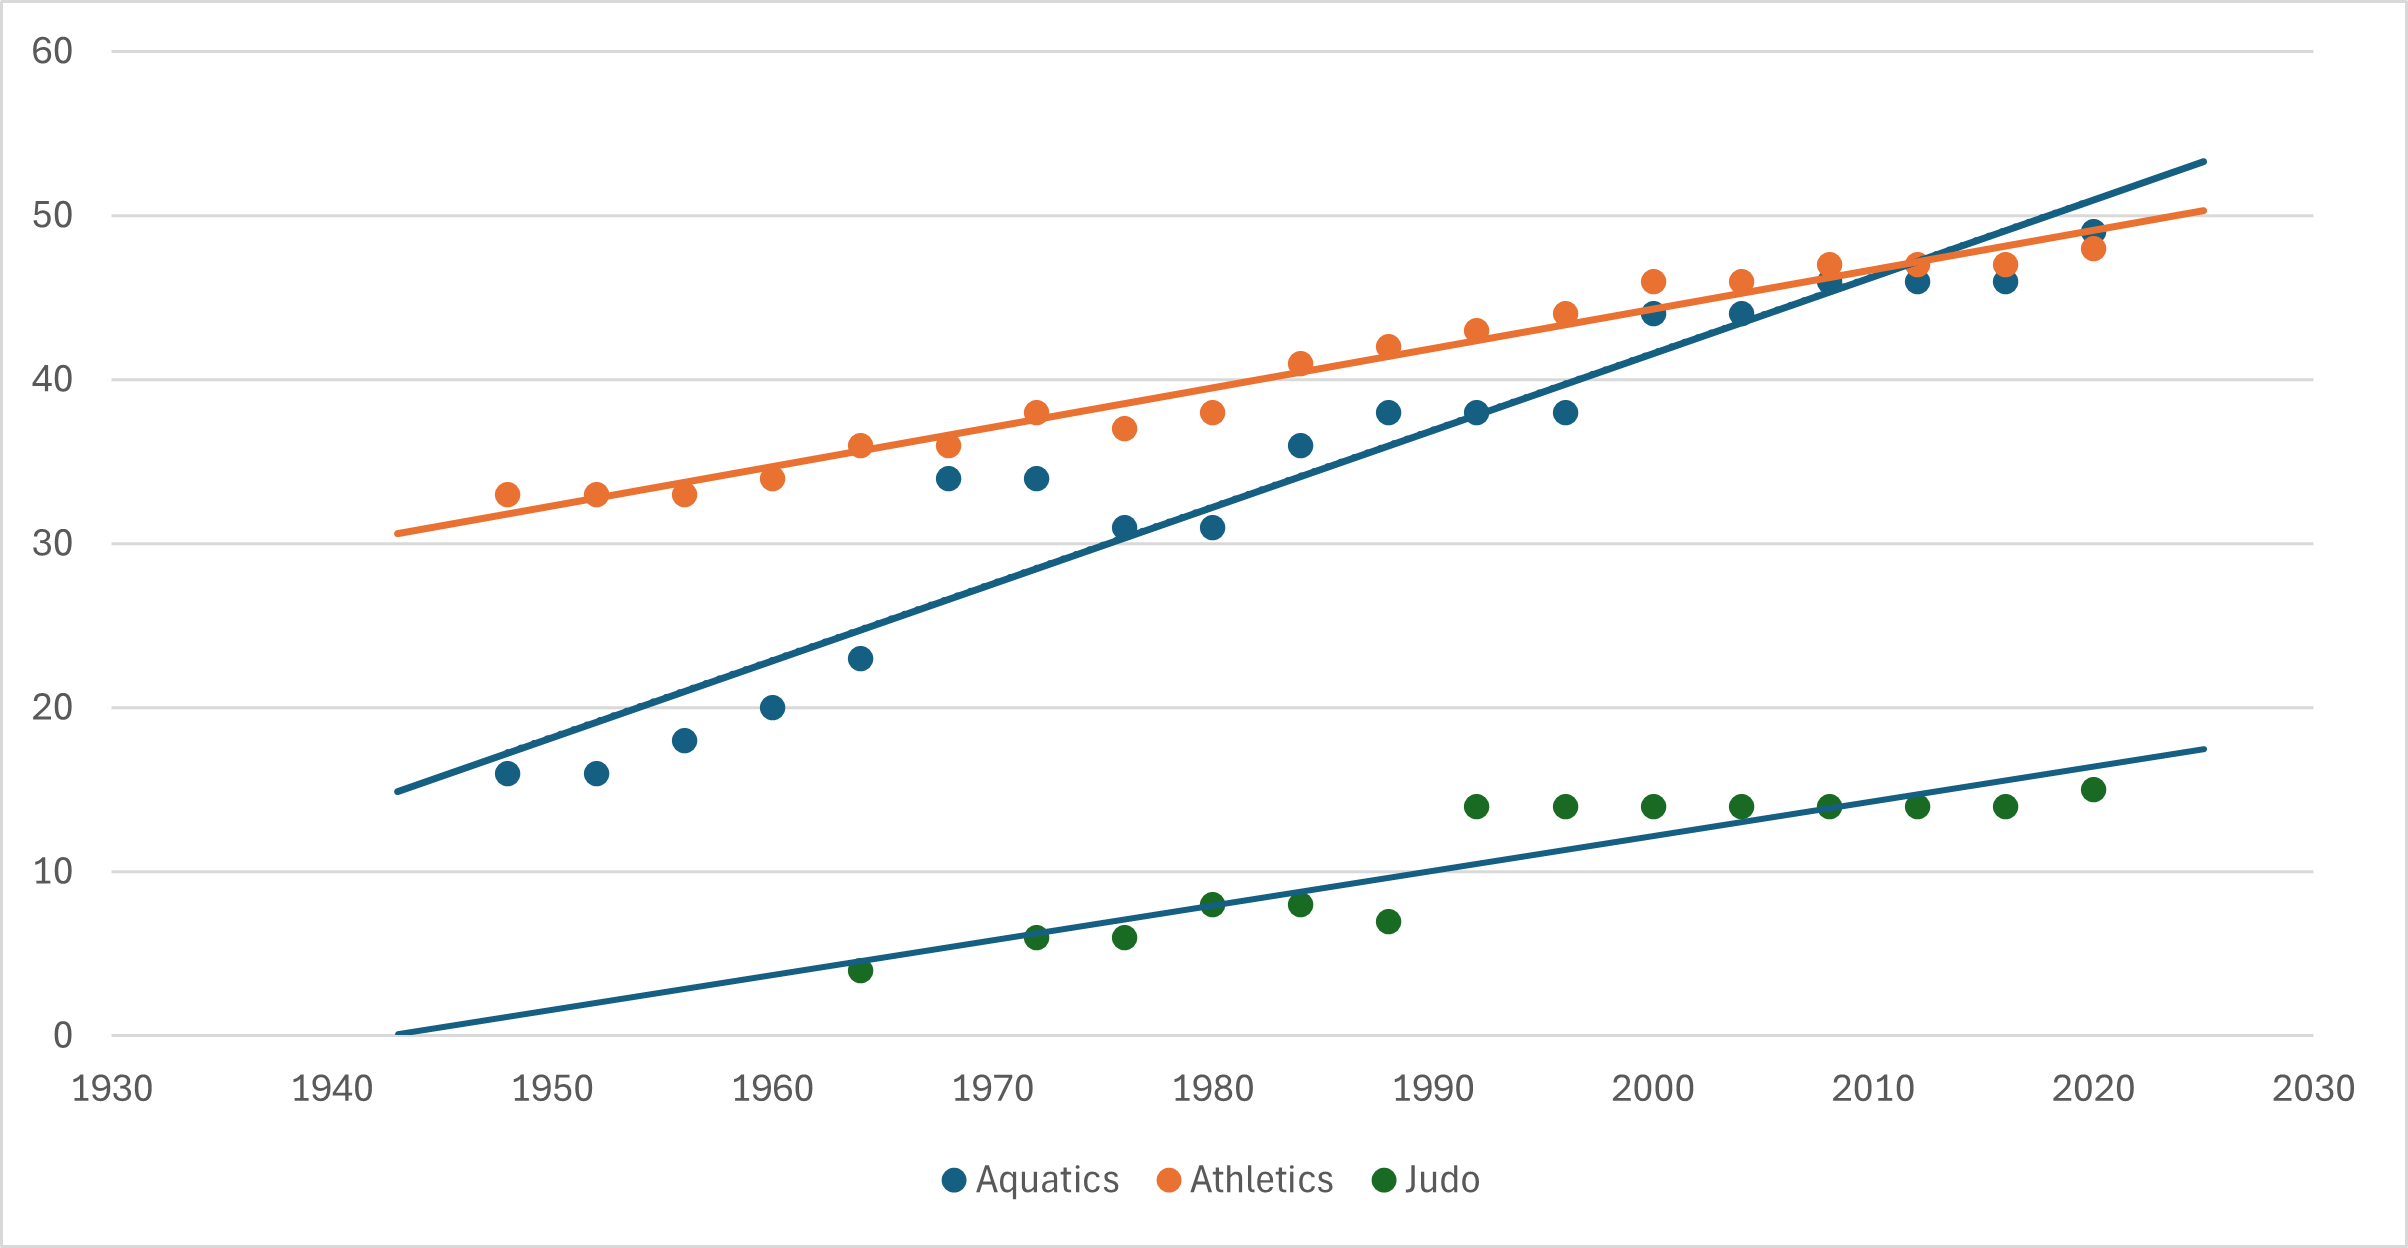
\includegraphics[width=0.8\textwidth]{图片1.png} %插入图片,[]中设置图片大小,{}中是图片文件名
    \caption{Main name 2} %最终文档中希望显示的图片标题
    \label{Fig.main2} %用于文内引用的标签
    \end{figure}
\begin{figure}[h] %H为当前位置,!htb为忽略美学标准,htbp为浮动图形
    \centering %图片居中
    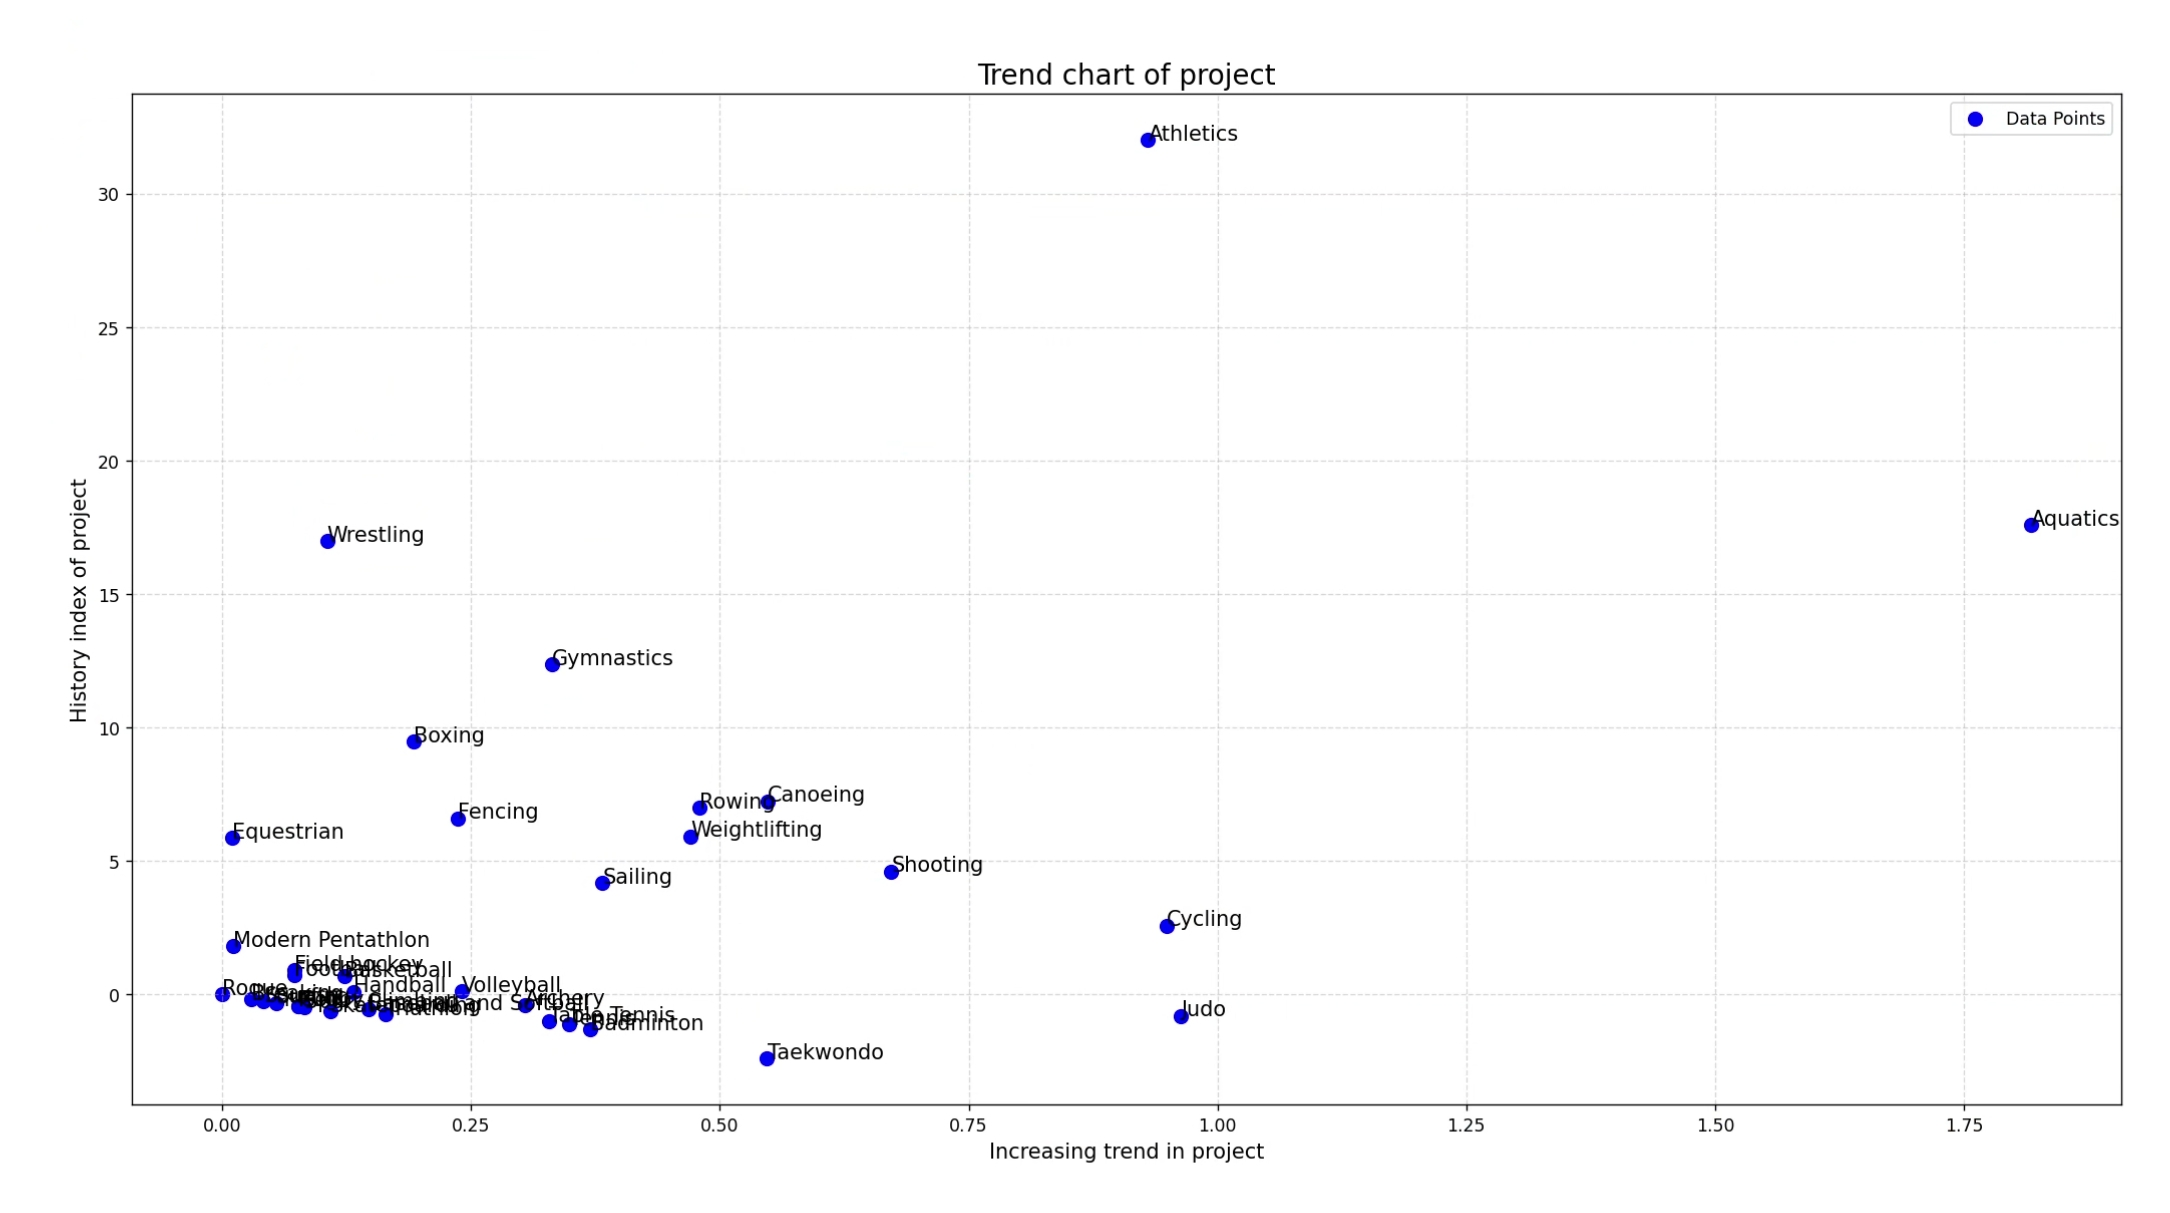
\includegraphics[width=0.8\textwidth]{TrendChartOfProject} %插入图片,[]中设置图片大小,{}中是图片文件名
    \caption{Main name 2} %最终文档中希望显示的图片标题
    \label{Fig.main2} %用于文内引用的标签
    \end{figure}


\section{Assumptions}
% 我们通过在网上查找多方面的资料并参考权威数据,最后对33个项目的七个维度进行了评分,结果如下:
% 展示表格
To simplify the problem, we make the following basic assumptions, each of which is
properly justified.
\begin{itemize}
\item[$\bullet$]Assumption 1: According to online information and authoritative data, 
we scored the 6 dimensions of 33 projects from 0~1 (1 means the best), and gave each project a weight for the possibility of creating more events. See Appendix for details.
\item[$\bullet$]Assumption 2:  No extreme events will occurr, such as war or natural disasters.
\end{itemize}
\section{Abbreviation and Definitions}
\section{The Evaluate Model}

\subsection{随机森林回归}
\subsubsection{Introduction}
%TODO: 随机森林回归的定义

我们以七个维度和作为自变量,线性拟合的斜率作为因变量,训练了一个随机森林回归模型。随机森林模型是一种基于决策树的模型,其本身是多个决策树并行的训练方式,有效地降低了训练的时间地同时带来更加精确的数据模型。该模型具有随机性强、不易overfit、对异常点outlier不敏感、适用于数据集中存在大量未知特征的情况、处理高维数据相对较快、能够估计哪个特征在分类中更重要、可以并行处理的优点,不过由于是黑盒,其不可解释的地方较多,在噪声过大的地方容易过拟合。
\subsubsection{Principle}
随机森林模型是基于决策树的,此处首先解释决策树选择最优决策的方法。此处引入熵的概念。\\
决策树是一种二叉树,每一层只做出一种选择,我们可以通过熵来衡量每一个父节点的不确定性。熵的计算公式如下:\\
$$H(X)= -\sum_{k=1}^N p_k log_2(p_k)$$
除去整一棵决策树的祖先,和最小的子节点,我们能算出每一个节点的熵的增益:
$$G(D)= H(X)-\sum_{v=1}^V \frac {\left|D^v\right|}{\left|D\right|} H(D)^v$$
其中G(D)表示熵的增益,H(X)表示上一层的熵,后面是当前一层的熵的总和。\\
决策树的整体流程如下:\\
(1) 过滤所有可能的决策条件。\\
(2) 选择子节点熵最小的决策条件。\\
(3) Repeat step1 and step2 until it reach the maximumpredefined depth or all the elements in a single lead node belong to one class.\\[1em]
接着来讲随机森林模型。随机森林模型首先从大量的数据中取样,然后构建多棵并行的决策树,基于决策树的熵最小决策原理得到每一棵树的最终决策,通过回归算法我们能用这些决策获得一个最终评测值,通过指定指标即可获得预测结果。
\subsubsection{Implementation}
We used the random forest fitting algorithm from the sklearn module of python.
% Code
\begin{listing}[htb]\caption{STH}\label{code:processdweet}
    \begin{minted}{python3}
        model = RandomForestRegressor(n_estimators=100, random_state=42)
        model.fit(X_train, y_train)
\end{minted} 
\end{listing}


\subsubsection{Result Analysis}
In the test set, our model achieved an R Square error of 0.6 and a mean square error of 0.12, making the regression training basically successful.

We used this model to predict data outside of the training and test sets

\begin{table}[]
    \begin{tabular}{lllllllll}
    Name      & Popularity and Accessibility & Gender Equity & Sustainability & Inclusivity & Relevance and Innovation & Safety and Fair Play & Basis & Rank        \\
    Wrestling & 0.7                          & 0.6           & 0.8            & 0.8         & 0.5                      & 0.8                  & 0     & 0.105263158 \\
              &                              &               &                &             &                          &                      &       &             \\
              &                              &               &                &             &                          &                      &       &            
    \end{tabular}
    \end{table}

结果表明,我们的模型在预测项目数量的增长上取得了成功。



\section{对SDE项目的预测}
我们对某个SDE项目进行了评分,输入我们的模型,得到了如下结果

我们认为 它的增长是xxx
\subsubsection{Background of This Problem}
\subsection{Efficiency and Robustness}
% \section{Sensitivity Analysis}
\section{Strengths and Weaknesses}
\subsection{Strengths}
\subsection{Weaknesses}
\section{Conclusion}
Hello world!test123
\section{Appendix}
\subsection{7-dimension Scores of the SDEs}
P.A. = Popularity and Accessibility \ G.E. = Gender Equality \ S. = Sustainability

I. = Inclusivity \ R.I. = Relevance and Innovation \ S.F. = Safety and Fair competition

M. = the possibility of creating More events
\begin{table*}[h]
    \begin{tabular}{|l|lllllll|l|ll}
    \cline{1-9}
    \multicolumn{1}{|c|}{\multirow{2}{*}{SDEs}} & \multicolumn{7}{c|}{Scores}                                                                                                                                                                                 & \multicolumn{1}{c|}{\multirow{2}{*}{Composite Scores}} &  &  \\ \cline{2-8}
    \multicolumn{1}{|c|}{}                      & \multicolumn{1}{c|}{P.A.}     & \multicolumn{1}{c|}{G.E.}     & \multicolumn{1}{c|}{S.}   & \multicolumn{1}{c|}{I.}   & \multicolumn{1}{c|}{R.I.} & \multicolumn{1}{c|}{S.F.}     & \multicolumn{1}{c|}{M.} & \multicolumn{1}{c|}{}                                  &  &  \\ \cline{1-9}
    Aquatics                                    & \multicolumn{1}{l|}{0.95}     & \multicolumn{1}{l|}{0.95}     & \multicolumn{1}{l|}{0.95} & \multicolumn{1}{l|}{0.95} & \multicolumn{1}{l|}{0.95} & \multicolumn{1}{l|}{0.95}     & 4                       & 1.817293                                               &  &  \\ \cline{1-9}
    Archery                                     & \multicolumn{1}{l|}{0.5}      & \multicolumn{1}{l|}{0.7}      & \multicolumn{1}{l|}{0.8}  & \multicolumn{1}{l|}{0.6}  & \multicolumn{1}{l|}{0.6}  & \multicolumn{1}{l|}{0.9}      & 0                       & 0.303759                                               &  &  \\ \cline{1-9}
    Athletics                                   & \multicolumn{1}{l|}{0.9}      & \multicolumn{1}{l|}{0.9}      & \multicolumn{1}{l|}{0.9}  & \multicolumn{1}{l|}{0.9}  & \multicolumn{1}{l|}{0.9}  & \multicolumn{1}{l|}{0.9}      & 0.6                     & 0.930075                                               &  &  \\ \cline{1-9}
    Badminton                                   & \multicolumn{1}{l|}{0.6}      & \multicolumn{1}{l|}{0.7}      & \multicolumn{1}{l|}{0.7}  & \multicolumn{1}{l|}{0.8}  & \multicolumn{1}{l|}{0.8}  & \multicolumn{1}{l|}{0.9}      & -2                      & 0.369925                                               &  &  \\ \cline{1-9}
    Baseball and Softball                       & \multicolumn{1}{l|}{0.65}     & \multicolumn{1}{l|}{0.65}     & \multicolumn{1}{l|}{0.7}  & \multicolumn{1}{l|}{0.6}  & \multicolumn{1}{l|}{0.65} & \multicolumn{1}{l|}{0.8}      & 1                       & 0.146617                                               &  &  \\ \cline{1-9}
    Basketball                                  & \multicolumn{1}{l|}{0.95}     & \multicolumn{1}{l|}{0.6}      & \multicolumn{1}{l|}{0.85} & \multicolumn{1}{l|}{0.85} & \multicolumn{1}{l|}{0.85} & \multicolumn{1}{l|}{0.6}      & -3                      & 0.122556                                               &  &  \\ \cline{1-9}
    Boxing                                      & \multicolumn{1}{l|}{0.7}      & \multicolumn{1}{l|}{0}        & \multicolumn{1}{l|}{1}    & \multicolumn{1}{l|}{0.4}  & \multicolumn{1}{l|}{0.5}  & \multicolumn{1}{l|}{0.2}      & 0                       & 0.192481                                               &  &  \\ \cline{1-9}
    Canoeing                                    & \multicolumn{1}{l|}{0.55}     & \multicolumn{1}{l|}{0.65}     & \multicolumn{1}{l|}{0.7}  & \multicolumn{1}{l|}{0.55} & \multicolumn{1}{l|}{0.6}  & \multicolumn{1}{l|}{0.8}      & 0                       & 0.54812                                                &  &  \\ \cline{1-9}
    Cycling                                     & \multicolumn{1}{l|}{0.8}      & \multicolumn{1}{l|}{0.75}     & \multicolumn{1}{l|}{0.8}  & \multicolumn{1}{l|}{0.68} & \multicolumn{1}{l|}{0.8}  & \multicolumn{1}{l|}{0.7}      & 0                       & 0.948872                                               &  &  \\ \cline{1-9}
    Equestrian                                  & \multicolumn{1}{l|}{0.4}      & \multicolumn{1}{l|}{0.7}      & \multicolumn{1}{l|}{0.7}  & \multicolumn{1}{l|}{0.5}  & \multicolumn{1}{l|}{0.5}  & \multicolumn{1}{l|}{0.74}     & -1.5                    & 0.009774                                               &  &  \\ \cline{1-9}
    Fencing                                     & \multicolumn{1}{l|}{0.6}      & \multicolumn{1}{l|}{0.7}      & \multicolumn{1}{l|}{0.8}  & \multicolumn{1}{l|}{0.6}  & \multicolumn{1}{l|}{0.7}  & \multicolumn{1}{l|}{0.9}      & 0                       & 0.236842                                               &  &  \\ \cline{1-9}
    Field hockey                                & \multicolumn{1}{l|}{0.7}      & \multicolumn{1}{l|}{0.8}      & \multicolumn{1}{l|}{0.8}  & \multicolumn{1}{l|}{0.7}  & \multicolumn{1}{l|}{0.7}  & \multicolumn{1}{l|}{0.9}      & -1.5                    & 0.07218                                                &  &  \\ \cline{1-9}
    Football                                    & \multicolumn{1}{l|}{1}        & \multicolumn{1}{l|}{0.9}      & \multicolumn{1}{l|}{0.9}  & \multicolumn{1}{l|}{1}    & \multicolumn{1}{l|}{0.9}  & \multicolumn{1}{l|}{1}        & -3                      & 0.07218                                                &  &  \\ \cline{1-9}
    Golf                                        & \multicolumn{1}{l|}{0.8}      & \multicolumn{1}{l|}{1}        & \multicolumn{1}{l|}{0.4}  & \multicolumn{1}{l|}{0.6}  & \multicolumn{1}{l|}{0.6}  & \multicolumn{1}{l|}{0.9}      & -2                      & 0.076692                                               &  &  \\ \cline{1-9}
    Gymnastics                                  & \multicolumn{1}{l|}{0.633333} & \multicolumn{1}{l|}{0.766667} & \multicolumn{1}{l|}{0.8}  & \multicolumn{1}{l|}{0.7}  & \multicolumn{1}{l|}{0.7}  & \multicolumn{1}{l|}{0.833333} & 0                       & 0.330827                                               &  &  \\ \cline{1-9}
    Handball                                    & \multicolumn{1}{l|}{0.65}     & \multicolumn{1}{l|}{0.65}     & \multicolumn{1}{l|}{0.8}  & \multicolumn{1}{l|}{0.6}  & \multicolumn{1}{l|}{0.7}  & \multicolumn{1}{l|}{0.85}     & -0.6                    & 0.131579                                               &  &  \\ \cline{1-9}
    Judo                                        & \multicolumn{1}{l|}{0.7}      & \multicolumn{1}{l|}{0.7}      & \multicolumn{1}{l|}{0.8}  & \multicolumn{1}{l|}{0.7}  & \multicolumn{1}{l|}{0.7}  & \multicolumn{1}{l|}{0.9}      & 1                       & 0.963158                                               &  &  \\ \cline{1-9}
    Rowing                                      & \multicolumn{1}{l|}{0.65}     & \multicolumn{1}{l|}{0.7}      & \multicolumn{1}{l|}{0.75} & \multicolumn{1}{l|}{0.65} & \multicolumn{1}{l|}{0.75} & \multicolumn{1}{l|}{0.85}     & 0                       & 0.478947                                               &  &  \\ \cline{1-9}
    Rugby                                       & \multicolumn{1}{l|}{0.75}     & \multicolumn{1}{l|}{0.75}     & \multicolumn{1}{l|}{0.8}  & \multicolumn{1}{l|}{0.75} & \multicolumn{1}{l|}{0.8}  & \multicolumn{1}{l|}{0.9}      & -2                      & 0.076692                                               &  &  \\ \cline{1-9}
    Sailing                                     & \multicolumn{1}{l|}{0.7}      & \multicolumn{1}{l|}{0.8}      & \multicolumn{1}{l|}{0.8}  & \multicolumn{1}{l|}{0.7}  & \multicolumn{1}{l|}{0.7}  & \multicolumn{1}{l|}{0.9}      & 0                       & 0.381955                                               &  &  \\ \cline{1-9}
    Shooting                                    & \multicolumn{1}{l|}{0.9}      & \multicolumn{1}{l|}{0.9}      & \multicolumn{1}{l|}{0.8}  & \multicolumn{1}{l|}{0.8}  & \multicolumn{1}{l|}{0.9}  & \multicolumn{1}{l|}{0.9}      & 0                       & 0.67218                                                &  &  \\ \cline{1-9}
    Skateboarding                               & \multicolumn{1}{l|}{0.8}      & \multicolumn{1}{l|}{0.9}      & \multicolumn{1}{l|}{0.8}  & \multicolumn{1}{l|}{0.7}  & \multicolumn{1}{l|}{0.8}  & \multicolumn{1}{l|}{0.8}      & 0                       & 0.108271                                               &  &  \\ \cline{1-9}
    Sport Climbing                              & \multicolumn{1}{l|}{0.3}      & \multicolumn{1}{l|}{0.4}      & \multicolumn{1}{l|}{0.7}  & \multicolumn{1}{l|}{0.4}  & \multicolumn{1}{l|}{0.4}  & \multicolumn{1}{l|}{0.6}      & 0                       & 0.082707                                               &  &  \\ \cline{1-9}
    Squash                                      & \multicolumn{1}{l|}{0.8}      & \multicolumn{1}{l|}{0.9}      & \multicolumn{1}{l|}{0.7}  & \multicolumn{1}{l|}{0.8}  & \multicolumn{1}{l|}{0.6}  & \multicolumn{1}{l|}{0.9}      & -1                      & 0.041353                                               &  &  \\ \cline{1-9}
    Surfing                                     & \multicolumn{1}{l|}{0.8}      & \multicolumn{1}{l|}{0.9}      & \multicolumn{1}{l|}{0.8}  & \multicolumn{1}{l|}{0.8}  & \multicolumn{1}{l|}{0.8}  & \multicolumn{1}{l|}{0.9}      & -2                      & 0.054135                                               &  &  \\ \cline{1-9}
    Table Tennis                                & \multicolumn{1}{l|}{0.9}      & \multicolumn{1}{l|}{0.9}      & \multicolumn{1}{l|}{0.8}  & \multicolumn{1}{l|}{0.8}  & \multicolumn{1}{l|}{0.9}  & \multicolumn{1}{l|}{0.9}      & -1                      & 0.32782                                                &  &  \\ \cline{1-9}
    Taekwondo                                   & \multicolumn{1}{l|}{0.4}      & \multicolumn{1}{l|}{0.4}      & \multicolumn{1}{l|}{0.6}  & \multicolumn{1}{l|}{0.4}  & \multicolumn{1}{l|}{0.5}  & \multicolumn{1}{l|}{0.7}      & 0                       & 0.547368                                               &  &  \\ \cline{1-9}
    Tennis                                      & \multicolumn{1}{l|}{0.6}      & \multicolumn{1}{l|}{0.6}      & \multicolumn{1}{l|}{0.8}  & \multicolumn{1}{l|}{0.6}  & \multicolumn{1}{l|}{0.6}  & \multicolumn{1}{l|}{0.8}      & 0                       & 0.348872                                               &  &  \\ \cline{1-9}
    Triathlon                                   & \multicolumn{1}{l|}{0.8}      & \multicolumn{1}{l|}{0.9}      & \multicolumn{1}{l|}{0.7}  & \multicolumn{1}{l|}{0.7}  & \multicolumn{1}{l|}{0.8}  & \multicolumn{1}{l|}{0.8}      & 0                       & 0.16391                                                &  &  \\ \cline{1-9}
    Volleyball                                  & \multicolumn{1}{l|}{0.6}      & \multicolumn{1}{l|}{0.6}      & \multicolumn{1}{l|}{0.8}  & \multicolumn{1}{l|}{0.6}  & \multicolumn{1}{l|}{0.6}  & \multicolumn{1}{l|}{0.8}      & -1                      & 0.240602                                               &  &  \\ \cline{1-9}
    Weightlifting                               & \multicolumn{1}{l|}{0.7}      & \multicolumn{1}{l|}{0.5}      & \multicolumn{1}{l|}{0.6}  & \multicolumn{1}{l|}{0.6}  & \multicolumn{1}{l|}{0.6}  & \multicolumn{1}{l|}{0.6}      & 0                       & 0.470677                                               &  &  \\ \cline{1-9}
    Wrestling                                   & \multicolumn{1}{l|}{0.7}      & \multicolumn{1}{l|}{0.6}      & \multicolumn{1}{l|}{0.8}  & \multicolumn{1}{l|}{0.8}  & \multicolumn{1}{l|}{0.5}  & \multicolumn{1}{l|}{0.8}      & 0                       & 0.105263                                               &  &  \\ \cline{1-9}
    Modern Pentathlon                           & \multicolumn{1}{l|}{0.5}      & \multicolumn{1}{l|}{0.6}      & \multicolumn{1}{l|}{0.7}  & \multicolumn{1}{l|}{0.6}  & \multicolumn{1}{l|}{0.7}  & \multicolumn{1}{l|}{0.7}      & 0                       & 0.010526                                               &  &  \\ \cline{1-9}
    Roque                                       & \multicolumn{1}{l|}{0.7}      & \multicolumn{1}{l|}{0.8}      & \multicolumn{1}{l|}{0.8}  & \multicolumn{1}{l|}{0.7}  & \multicolumn{1}{l|}{0.8}  & \multicolumn{1}{l|}{0.9}      & 0                       & 0.3                                                    &  &  \\ \cline{1-9}
    \end{tabular}
    \end{table*}
\end{document}  